\documentclass[runningheads]{llncs}

\usepackage{amsmath}
\usepackage{booktabs}
\usepackage{amssymb}
\usepackage{graphicx}
\usepackage[square,numbers]{natbib}
\usepackage[utf8]{inputenc}
\usepackage{hyperref}
\usepackage[margin=1.2in]{geometry}
\usepackage{placeins}

\renewcommand{\topfraction}{0.85}
\renewcommand{\bottomfraction}{0.85}
\renewcommand{\textfraction}{0.10}
\renewcommand{\floatpagefraction}{0.80}
\setlength{\floatsep}{3pt plus 1pt minus 1pt}
\setlength{\textfloatsep}{3pt plus 1pt minus 1pt}
\setlength{\intextsep}{3pt plus 1pt minus 1pt}
\setlength{\abovecaptionskip}{2pt plus 1pt minus 1pt}

\begin{document}

\title{Spectral Analysis of U.S.\ Equity Markets:\\
Factor Structure, Sectoral Geometry, and Market Efficiency}

\author{Damon H.\,T.\ Cheung}
\institute{University of Michigan, Ann Arbor, MI 48109}

\maketitle

\begin{abstract}
We apply spectral and data-driven methods to daily returns of 20 large-cap
U.S.\ equities (2020--2026) to ask: how many independent directions of variation
does the market possess, and can that structure be exploited for prediction?
Singular Value Decomposition (SVD) reveals only four statistically genuine factors;
Classical Multidimensional Scaling (MDS) and Spectral Clustering recover the four
known sectors without any labels.
Dynamic Mode Decomposition (DMD) shows that returns are temporally unpredictable—a
trained linear model underperforms a zero-change forecast, and a portfolio acting
on its predictions loses $-45.4\%$ while the passive benchmark gains $+92.0\%$.
Generalized Autoregressive Conditional Heteroskedasticity (GARCH) modelling shows
the complementary result: while return \emph{direction} is unpredictable, return
\emph{magnitude} (volatility) is forecastable, and a volatility-targeting portfolio
achieves $+96.4\%$ with a higher Sharpe ratio.
The market is low-dimensional across stocks yet unpredictable in time—the
mathematical signature of market efficiency.
\end{abstract}


% ──────────────────────────────────────────────────────────────────────────────
\section{Introduction}
% ──────────────────────────────────────────────────────────────────────────────

The U.S.\ equity market is one of the most intensively studied dynamical systems
in the world—and one of the most difficult to predict \citep{fama1970efficient}.
Yet most stocks move together: when the broad market falls, individual stocks
fall with it regardless of their fundamentals.
This co-movement raises a precise mathematical question:
\emph{how many independent directions of variation does the equity return matrix
truly possess, and does this structure enable prediction?}

We address this question by applying SVD, Classical MDS, Spectral Clustering,
Dynamic Mode Decomposition (DMD), and GARCH to daily returns of 20 large-cap
U.S.\ stocks over 2020--2026.
Our central finding resolves an apparent paradox:
\emph{the market is low-dimensional across stocks but unpredictable over time.}
SVD reveals four genuine factors that spectral methods recover exactly from raw
returns; DMD shows this structure cannot be extrapolated forward; GARCH shows
that \emph{volatility} can be forecast even when return direction cannot.
The implication: mathematical methods can characterise market structure and
manage risk, but cannot predict direction.


% ──────────────────────────────────────────────────────────────────────────────
\section{Data and Methods}
% ──────────────────────────────────────────────────────────────────────────────

\paragraph{Data.}
We use daily adjusted closing prices from Yahoo Finance for 20 large-cap U.S.\
stocks, five from each of four sectors—Technology (AAPL, MSFT, GOOGL, AMZN,
META), Finance (JPM, BAC, GS, MS, C), Healthcare (JNJ, UNH, PFE, MRK, ABBV),
and Energy (XOM, CVX, COP, SLB, EOG)—plus the S\&P~500 index as an external
benchmark.
The period is 2 January 2020 to 24 April 2026 ($T = 1{,}585$ trading days,
$N = 20$ stocks).
We compute daily log-returns $r_{i,t} = \ln(p_{i,t}/p_{i,t-1})$ and standardise
each stock to zero mean and unit variance, yielding the return matrix
$\mathbf{X} \in \mathbb{R}^{T \times N}$.

\paragraph{SVD and Random-Matrix Baseline.}
We compute the thin SVD
\begin{equation}
  \mathbf{X} = \mathbf{U}\boldsymbol{\Sigma}\mathbf{V}^\top,\qquad
  \boldsymbol{\Sigma}=\mathrm{diag}(\sigma_1\geq\cdots\geq\sigma_N\geq 0),
  \label{eq:svd}
\end{equation}
whose right singular vectors (columns of $\mathbf{V}$) are the principal
components; the $k$-th explains variance fraction $\sigma_k^2/\sum_j\sigma_j^2$.
To separate genuine factors from finite-sample noise we apply the
Mar\v{c}enko--Pastur law \citep{marchenko1967distribution}: for an i.i.d.\
Gaussian matrix with aspect ratio $q=N/T$, bulk eigenvalues are bounded by
\begin{equation}
  \lambda_{\pm} = \bigl(1\pm\sqrt{q}\,\bigr)^2;
  \label{eq:mp}
\end{equation}
eigenvalues above $\lambda_+$ signal statistically genuine structure.

\paragraph{Correlation, MDS, and Spectral Clustering.}
We form the $20\times20$ Pearson correlation matrix $\mathbf{C}$, where
\begin{equation}
  \rho_{ij} = \frac{\sum_{t}(r_{i,t}-\bar r_i)(r_{j,t}-\bar r_j)}
    {\sqrt{\sum_t(r_{i,t}-\bar r_i)^2\cdot\sum_t(r_{j,t}-\bar r_j)^2}}
  \label{eq:pearson}
\end{equation}
is the pairwise return correlation (which simplifies to
$\rho_{ij}=\tfrac{1}{T-1}\sum_t r_{i,t}r_{j,t}$ after standardisation).
Classical MDS \citep{kutz2016dynamic} embeds stocks in $\mathbb{R}^2$ via the
correlation distance $d_{ij}=\sqrt{2(1-\rho_{ij})}$.
Spectral clustering \citep{luxburg2007tutorial} with $k=4$ (motivated by the
four clusters visible in the MDS embedding) uses $\tfrac{1}{2}(\mathbf{C}+\mathbf{1})$
as an affinity matrix; we evaluate it with the Adjusted Rand Index
(ARI; $1$ = perfect agreement, $0$ = chance).

\paragraph{Dynamic Mode Decomposition and Portfolio Test.}
DMD finds the best rank-$r$ linear map satisfying
$\mathbf{x}_{t+1}\approx\mathbf{A}\mathbf{x}_t$ \citep{kutz2016dynamic}.
Given snapshot matrices $\mathbf{X}_1,\mathbf{X}_2\!\in\!\mathbb{R}^{N\times(T-1)}$
and a rank-$r$ SVD $\mathbf{X}_1=\mathbf{U}_r\boldsymbol{\Sigma}_r\mathbf{V}_r^\top$,
the reduced operator and its full-space reconstruction are
\begin{equation}
  \tilde{\mathbf{A}}=\mathbf{U}_r^\top\mathbf{X}_2\mathbf{V}_r\boldsymbol{\Sigma}_r^{-1},
  \qquad
  \mathbf{A}=\mathbf{U}_r\tilde{\mathbf{A}}\mathbf{U}_r^\top.
  \label{eq:dmd}
\end{equation}
We sweep $r=1,\ldots,N$ to examine whether any truncation level recovers
latent predictability; results for $r=N=20$ (full rank) serve as the main
reference since they give DMD maximum information.
We train on 2020--2022 (755 days) and test on 2023--2026 (830 days).
Predictability is measured by the RMSE ratio $\mathrm{RMSE}_{\hat A}/\mathrm{RMSE}_{0}$
(ratio $>1$: the model is worse than predicting no change), and by a
dollar-neutral long-short portfolio
\begin{equation}
  r_t^{\text{port}} = \frac{1}{10}\!\sum_{i\in\mathcal{L}_t}\!r_{i,t}
    - \frac{1}{10}\!\sum_{i\in\mathcal{S}_t}\!r_{i,t},
  \label{eq:portfolio}
\end{equation}
where $\mathcal{L}_t$ ($\mathcal{S}_t$) is the 10 highest (lowest) predicted-return
stocks on day $t$, tracked against an equal-weight buy-and-hold benchmark.

\paragraph{GARCH Volatility Modelling and Volatility-Targeting Portfolio.}
Having shown that DMD cannot predict return \emph{direction}, we ask whether
return \emph{magnitude} (volatility) is forecastable.
We fit a GARCH(1,1) model \citep{bollerslev1986generalized} to S\&P~500 returns:
\begin{equation}
  r_t = \varepsilon_t\sqrt{h_t},\qquad
  h_t = \omega + \alpha\,r_{t-1}^2 + \beta\,h_{t-1},
  \label{eq:garch}
\end{equation}
where $h_t$ is the conditional variance, $\alpha$ captures the immediate shock
impact, and $\beta$ governs persistence.
We evaluate the one-step-ahead volatility forecast on the 2023--2026 test set
against the unconditional-mean baseline.
We also construct a \emph{volatility-targeting} portfolio whose daily position
size $w_t = \min(\sigma^*/\hat\sigma_t,\,2)$ scales the equal-weight portfolio to
a target daily volatility $\sigma^*=1\%$, capping leverage at $2\times$.
Performance throughout is summarised by the annualised Sharpe ratio
$\mathrm{SR}=(\bar r_d/\hat\sigma_d)\sqrt{252}$.
As a robustness check we also fit GARCH(1,1) to each of the 20 stocks
individually, isolating idiosyncratic from systematic variance.


% ──────────────────────────────────────────────────────────────────────────────
\section{Results}
% ──────────────────────────────────────────────────────────────────────────────

\subsection{The Market Is Low-Dimensional: Four Genuine Factors}

\begin{figure}[t]
  \centering
  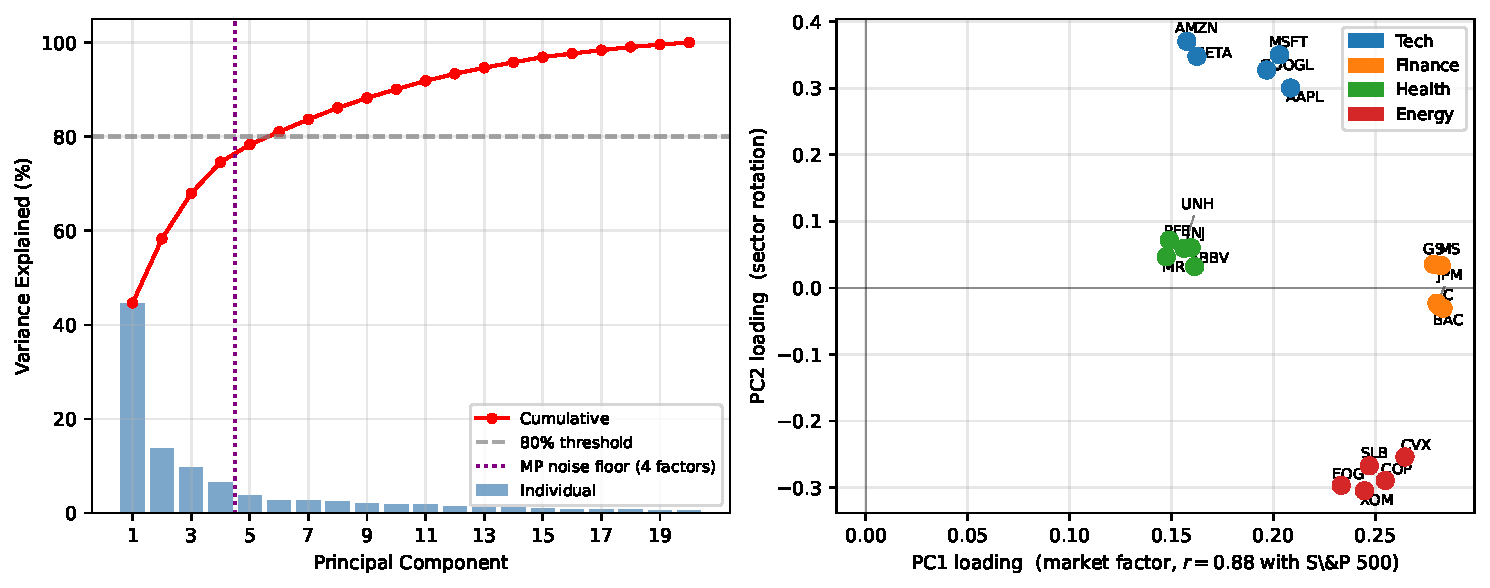
\includegraphics[width=\linewidth]{figures/fig1_svd.pdf}
  \caption{SVD of the standardised return matrix $\mathbf{X}$.
  \textbf{(a)} Scree plot: the dotted vertical line marks the
  Marchenko--Pastur noise floor; only four eigenvalues exceed it.
  \textbf{(b)} Stock loadings on PC1 vs.\ PC2.
  Every stock has a positive PC1 loading (the market factor);
  PC2 separates Energy and Finance from Technology.}
  \label{fig:svd}
\end{figure}

PC1 captures 44.6\% of total variance; the top three PCs together explain
67.9\%.
Crucially, the Marchenko--Pastur bound $\lambda_+=1.24$ is exceeded by
exactly \emph{four} eigenvalues (Fig.~\ref{fig:svd}a)—all remaining 16 are
statistically indistinguishable from random noise.
The market is genuinely low-dimensional: a $20$-stock universe reduces to
four meaningful directions.

Figure~\ref{fig:svd}b shows what those directions are.
Every stock has a positive PC1 loading, confirming a single market-wide
co-movement factor ($r=0.883$ with the S\&P~500 index)—the market factor of
\citet{fama1993common}.
PC2 then separates Energy and Finance from Technology, hinting that the
remaining factors capture sector-specific variation.

\subsection{Sector Structure Is Perfectly Recoverable Without Labels}

\begin{figure}[t]
  \centering
  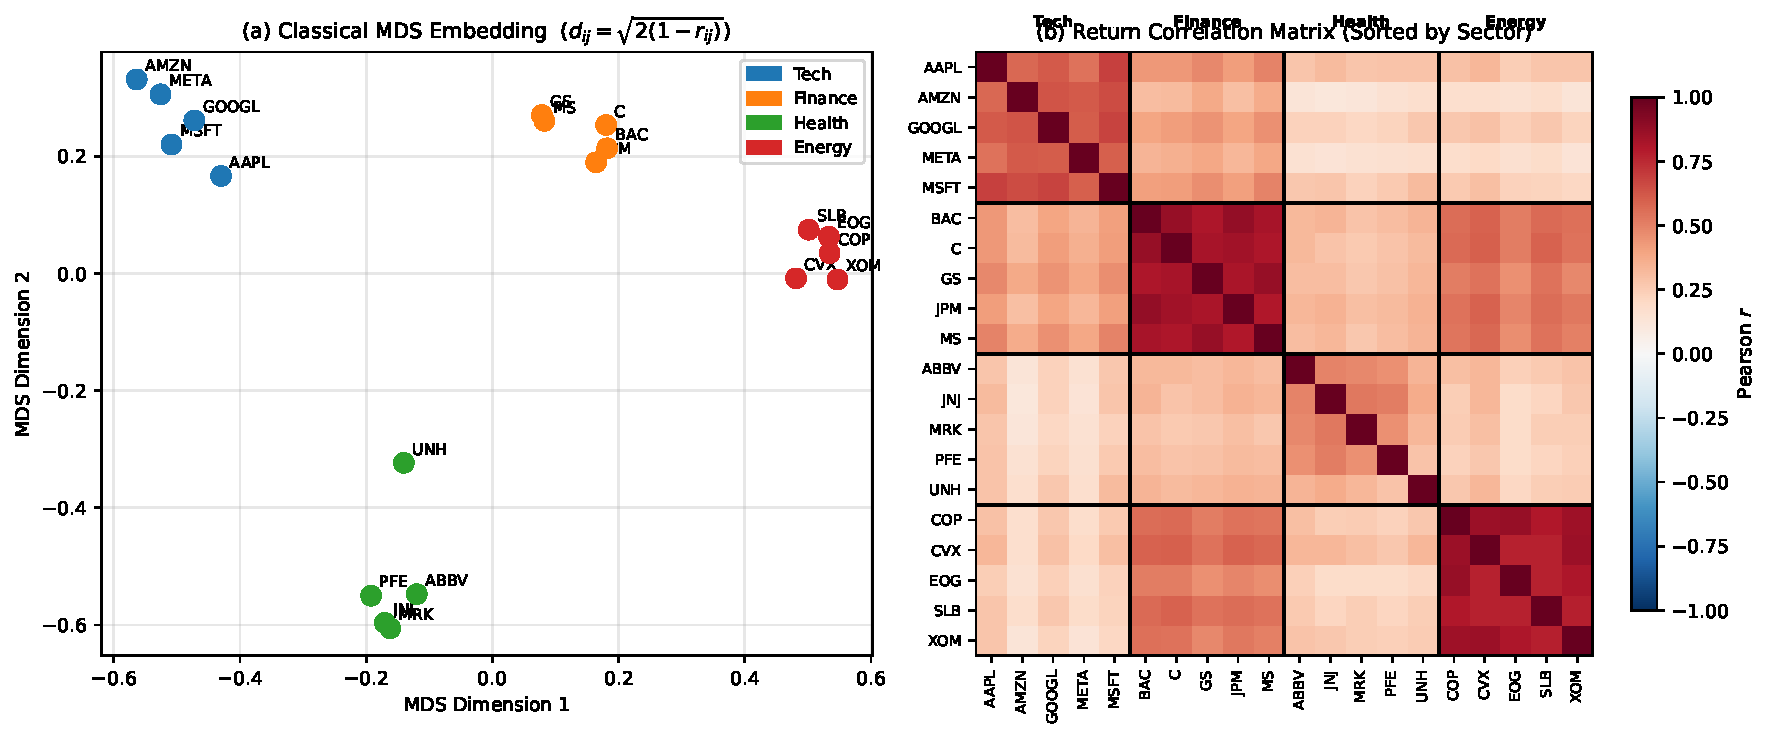
\includegraphics[width=\linewidth]{figures/fig2_structure.pdf}
  \caption{\textbf{(a)} Classical MDS embedding: stocks cluster by sector
  with no label information supplied.
  \textbf{(b)} Pearson correlation matrix sorted by sector.
  Within-sector blocks are warm (high $\rho_{ij}$); cross-sector blocks are cool.}
  \label{fig:structure}
\end{figure}

The MDS embedding (Fig.~\ref{fig:structure}a) translates correlation geometry
into Euclidean space: Technology clusters tightly in the upper region, Energy
to the lower left, with Finance and Healthcare in between.
No sector labels were provided—the geometry emerges entirely from return
correlations.

Spectral clustering with $k=4$ reproduces the known sector partition exactly
(ARI $=1.00$), supported by the block-diagonal structure of the correlation
heatmap (Fig.~\ref{fig:structure}b).
Within-sector correlations are consistently higher than cross-sector ones;
Technology--Technology pairs are the most tightly linked, while
Energy--Technology pairs are the most decorrelated.

\emph{What we learned:} the four-factor structure found by SVD maps directly
onto the four economic sectors.
The market is not just low-dimensional—it is \emph{interpretably}
low-dimensional.

\subsection{Returns Are Temporally Unpredictable: DMD Fails}

\begin{figure}[t]
  \centering
  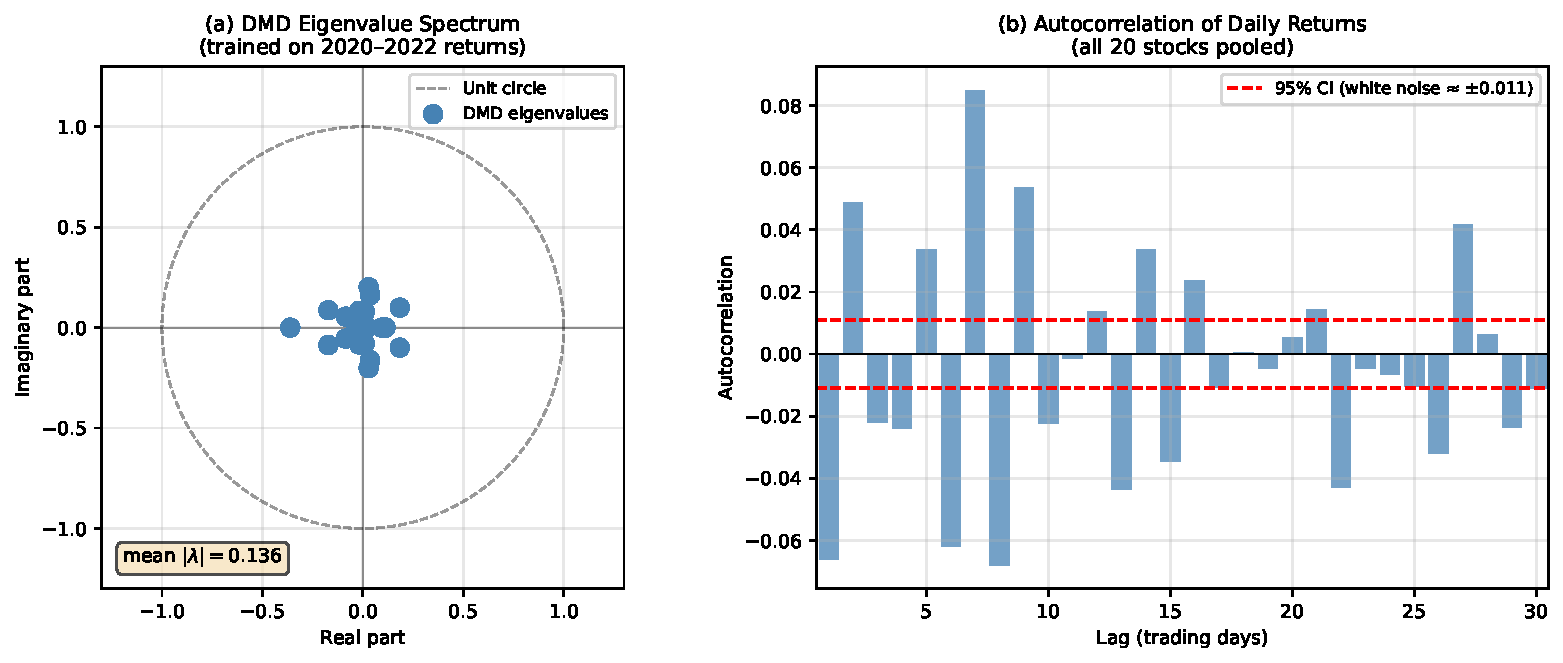
\includegraphics[width=\linewidth]{figures/fig3_dmd.pdf}
  \caption{\textbf{(a)} DMD eigenvalue spectrum (trained 2020--2022,
  tested 2023--2026). All eigenvalues lie well inside the unit circle
  (mean $|\lambda|=0.136$), indicating modes that decay within one trading day.
  \textbf{(b)} Lag-$k$ autocorrelation $\rho_k=\mathrm{Corr}(r_t,r_{t-k})$:
  nearly every bar is within the 95\% white-noise band (red dashes).
  \textbf{(c)} The DMD long-short portfolio loses $-45.4\%$ over the test
  period while the equal-weight benchmark gains $+92.0\%$.}
  \label{fig:dmd}
\end{figure}

Having established that the market's cross-sectional structure is
low-dimensional, we now ask whether that structure can be extrapolated forward
in time.
DMD finds the answer in its eigenvalues: all 20 lie well inside the unit circle
(mean $|\lambda|=0.136$, Fig.~\ref{fig:dmd}a).
In systems with persistent dynamics—such as fluid oscillations—DMD eigenvalues
sit \emph{on} the unit circle and encode stable modes that can be tracked.
Here every mode decays within a single trading day; there is no dynamical
backbone to extrapolate.

This failure is confirmed statistically and economically.
Statistically, the lag-$k$ autocorrelation $\rho_k=\mathrm{Corr}(r_t,r_{t-k})$
measures whether today's return predicts tomorrow's: values near zero for all
$k\geq1$ indicate white noise (Fig.~\ref{fig:dmd}b).
The only exception is a small negative $\rho_1=-0.066$, a well-known
microstructure artefact (bid-ask bounce) that vanishes after transaction costs.
Economically, a DMD model trained on 2020--2022 achieves an out-of-sample RMSE
of $0.762$ vs.\ the zero-change baseline of $0.735$ (ratio $1.04$)—the trained
model is \emph{worse} than predicting no change.
A portfolio acting on these predictions loses $-45.4\%$ over the 2023--2026 test
period, while a passive equal-weight portfolio gains $+92.0\%$
(Fig.~\ref{fig:dmd}c, annualised Sharpe $=-1.23$).

\paragraph{Rank sensitivity.}
To test whether a lower-rank truncation recovers latent predictability, we
evaluate DMD for every $r=1,\ldots,20$ (Fig.~\ref{fig:dmd_rank}).
Two results stand out.
First, RMSE increases monotonically with $r$: adding noise modes strictly hurts
out-of-sample prediction, with no elbow or optimal interior rank.
Second, the best long-short portfolio return is achieved at $r=3$
($+49.0\%$, Sharpe $=0.80$)---precisely the number of eigenvalues that
exceed the Mar\v{c}enko--Pastur noise floor.
This alignment is not coincidental: the three genuine cross-sectional factors
provide the cleanest signal for relative stock ranking.
Yet even at this optimal $r$, the strategy returns less than half the passive
benchmark ($+92.0\%$, Sharpe $=1.43$).
Above $r=3$ the additional modes are noise, and portfolio returns collapse;
at $r=1$ the single market factor predicts all stocks moving together,
rendering the long-short ranking useless ($-46.0\%$).
The rank sweep therefore sharpens the earlier finding: the
market's cross-sectional structure is exploitable only at the factor level,
and even then not enough to beat the market.

\begin{figure}[t]
  \centering
  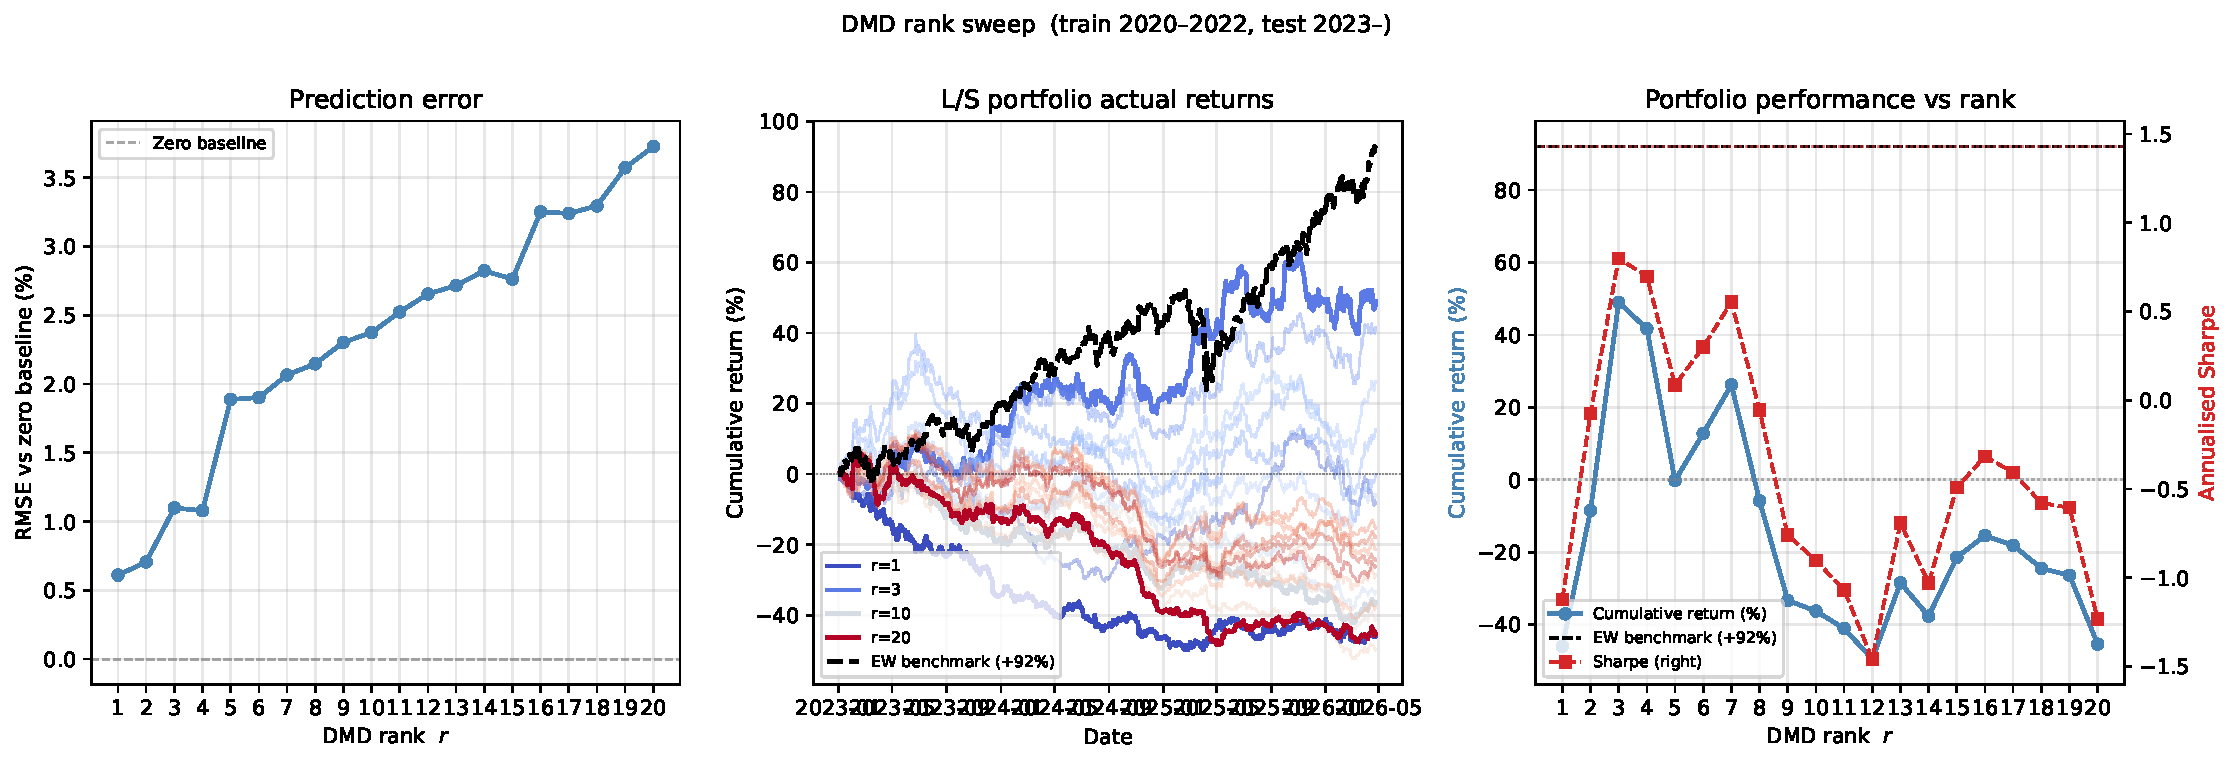
\includegraphics[width=\linewidth]{figures/fig_dmd_rank_sweep.pdf}
  \caption{DMD rank sweep ($r=1,\ldots,20$), trained 2020--2022 and tested 2023--2026.
  \textbf{(a)} One-step RMSE penalty relative to the zero-change baseline: every rank
  is worse than predicting no change, and the penalty grows with $r$.
  \textbf{(b)} Cumulative L/S portfolio returns for each $r$ (coloured) vs.\ the
  equal-weight benchmark (dashed black).
  \textbf{(c)} Summary of cumulative return and annualised Sharpe by rank; the
  optimum at $r=3$ coincides with the Mar\v{c}enko--Pastur noise-floor count.}
  \label{fig:dmd_rank}
\end{figure}

\emph{What we learned:} the market's stable spatial structure does not imply
temporal predictability.
Any linear pattern in returns is arbitraged away before it can be exploited—the
mathematical signature of the Efficient Market Hypothesis
\citep{fama1970efficient}.

\subsection{Volatility Is Predictable: GARCH Succeeds Where DMD Fails}

\begin{figure}[t]
  \centering
  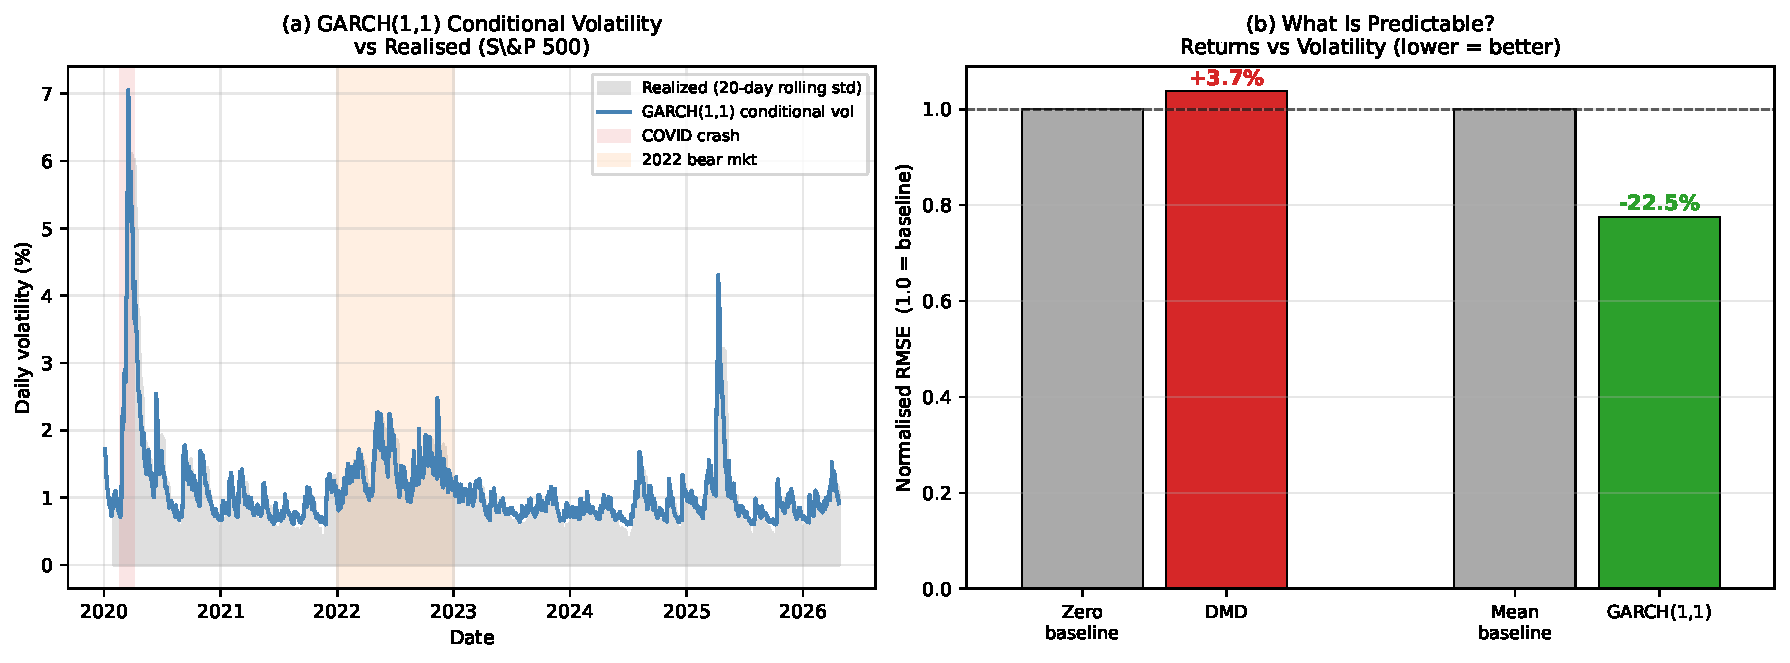
\includegraphics[width=\linewidth]{figures/fig4_garch.pdf}
  \caption{\textbf{(a)} GARCH(1,1) conditional volatility vs.\ realised
  absolute returns (S\&P~500). The model tracks the COVID-19 crash (Mar.\ 2020)
  and the 2022 rate-hike sell-off.
  \textbf{(b)} Normalised RMSE: DMD predicts \emph{returns} worse than the
  zero baseline (ratio $>1$); GARCH predicts \emph{volatility} substantially
  better than the historical mean (ratio $<1$).}
  \label{fig:garch}
\end{figure}

The DMD result establishes that the first moment of returns (expected value) is
unpredictable.
We now ask whether the second moment (variance) is equally featureless.
Fitting GARCH(1,1) to S\&P~500 returns yields $\hat\alpha=0.158$ and
$\hat\beta=0.804$, giving persistence $\hat\alpha+\hat\beta=0.962$.
This near-unity persistence means a large volatility shock today still echoes
strongly tomorrow—volatility is long-lived and therefore forecastable.
The model achieves a 22.5\% reduction in RMSE on the held-out 2023--2026 period
relative to predicting the historical mean (Fig.~\ref{fig:garch}b).
Applied stock-by-stock to the 20 individual equities, GARCH barely improves on
the unconditional mean (8 of 20 stocks, mean RMSE ratio $1.005$): the forecastable
component is \emph{systematic} market volatility (captured by the S\&P~500
index), not idiosyncratic variance.
In portfolio terms, a GARCH volatility-targeting strategy ($+96.4\%$,
Sharpe $=1.44$) modestly outperforms the passive benchmark ($+92.0\%$,
Sharpe $=1.43$) by scaling exposure up during calm periods and down during
high-volatility episodes—contrasting sharply with the DMD long-short strategy
($-45.4\%$, Sharpe $=-1.23$) that catastrophically underperforms the same
benchmark.

\emph{What we learned:} the EMH constrains the predictability of return
\emph{direction} (first moment), not return \emph{magnitude} (second moment).
Mathematical methods can manage risk but not manufacture alpha.


% ──────────────────────────────────────────────────────────────────────────────
\section{Conclusion}
% ──────────────────────────────────────────────────────────────────────────────
\typeout{AFTER SECTION: pagegoal=\the\pagegoal, pagetotal=\the\pagetotal}

\emph{So what?}
We set out to ask whether the U.S.\ equity market is low-dimensional, and whether
that structure enables prediction.
The answer is: \emph{yes to the first, no—and yes—to the second, depending on
what you try to predict.}

Across stocks, the market is organised into exactly four statistically genuine
factors that align perfectly with the four economic sectors.
This structure is stable, interpretable, and recoverable without labels—a
mathematical counterpart of the Fama--French factor model \citep{fama1993common}.

Over time, return \emph{direction} is not predictable.
DMD's eigenvalues cluster at the origin rather than on the unit circle.
A systematic rank sweep reveals that the optimal truncation is $r=3$—matching
the Mar\v{c}enko--Pastur noise floor—yet even this best case returns only
$+49.0\%$ (Sharpe $=0.80$) against the passive benchmark's $+92.0\%$
(Sharpe $=1.43$); at full rank ($r=20$) the portfolio loses $45.4\%$.
Any learnable pattern in prices is immediately arbitraged away—the mathematical
signature of the Efficient Market Hypothesis \citep{fama1970efficient}.
Return \emph{magnitude}, however, is predictable: GARCH captures volatility
persistence ($\hat\alpha+\hat\beta=0.962$), reduces forecasting error by 22.5\%,
and enables a risk-adjusted strategy that outperforms the benchmark.

The take-away is precise: invest in risk management, not in return-prediction
algorithms—spectral methods expose the boundary between what can and cannot
be predicted with mathematical clarity.
\typeout{END OF CONCLUSION: pagegoal=\the\pagegoal, pagetotal=\the\pagetotal, remaining=\the\dimexpr\pagegoal-\pagetotal}

\begin{thebibliography}{1}
\providecommand{\url}[1]{\texttt{#1}}
\providecommand{\urlprefix}{URL }
\providecommand{\doi}[1]{https://doi.org/#1}

\bibitem{bollerslev1986generalized}
Bollerslev, T.: Generalized autoregressive conditional heteroskedasticity.
  Journal of Econometrics  \textbf{31}(3),  307--327 (1986)

\bibitem{fama1970efficient}
Fama, E.F.: Efficient capital markets: {A} review of theory and empirical work.
  The Journal of Finance  \textbf{25}(2),  383--417 (1970)

\bibitem{fama1993common}
Fama, E.F., French, K.R.: Common risk factors in the returns on stocks and
  bonds. Journal of Financial Economics  \textbf{33}(1),  3--56 (1993)

\bibitem{kutz2016dynamic}
Kutz, J.N., Brunton, S.L., Brunton, B.W., Proctor, J.L.: Dynamic Mode
  Decomposition: Data-Driven Modeling of Complex Systems. SIAM, Philadelphia
  (2016)

\bibitem{marchenko1967distribution}
Mar{\v{c}}enko, V.A., Pastur, L.A.: Distribution of eigenvalues for some sets
  of random matrices. Mathematics of the USSR-Sbornik  \textbf{1}(4),  457--483
  (1967)

\bibitem{luxburg2007tutorial}
Von~Luxburg, U.: A tutorial on spectral clustering. Statistics and Computing
  \textbf{17}(4),  395--416 (2007)

\end{thebibliography}

\end{document}
